\documentclass[11pt]{article}

\usepackage{microtype}
\usepackage{amsmath}
\usepackage{xcolor}
\usepackage{graphicx}
\usepackage{enumitem}


\setlength{\parindent}{0cm}
\renewcommand\thesubsection{\alph{subsection})}

\title{\textbf{Assignment 1\\}Search Algorithms}
\author{Malik Al-hallak 90020\\
		Sebastian Utzig 100059\\
		Clemens Wegener 91268}
\date{}
\begin{document}

\maketitle
\section{Computational complexity theory}

\setcounter{subsection}{1} %counter manuell erhöhen
\subsection{}
$f(n) = \Omega{(g(n))} \Longleftrightarrow \exists\: c>0,\exists \: n_0>0:c\cdot |g(n)|\leq|f(n)|$

\section{Computational complexity theory}
\subsection{}
\emph{Computational Model}: NP problems can be solved by a non-deterministic Turing machine in polynomial time.

\bigskip

\emph{Ressource Limit}: \begin{itemize}[nosep]
							\item computational time
							\item \# of steps for solution
							\item memory 
						\end{itemize}

\subsection{}
NP-Hard problems define a class of problems whose solution algorithm working in polynomial time leads to a polynomial solution algorithm for problems in NP. Vice versa all problems in NP can be reduced to NP-Hard problems.

\subsection{}
Every NP-Hard Problem classified as NP is said to be NP-Complete.

\subsection{}
Since the left side of all production rules only contains single non-terminals it is said to be context-free.

At the same time \emph{G} is not regular (Type-3) due to multiple terminals and non-terminals on the right side of the production rules.

Therefore, the presented context-free non-regular grammar \emph{G} is of Type-2.

\section{Computational complexity theory}
\subsection{}
The 3-SAT problem is a boolean satisfiability problem. 

Given a formula in conjunctive normal form where each clause is limited to at most three literals, finding a configuration for the variables for which the formula evaluates to TRUE is NP-Complete. An \emph{instance} is for example:
\begin{equation*}
%TODO Strich drüber !!!
	F=(x_1 \lor \lnot x_2\lor x_3)\land(x_2\lor x_3 \lor \lnot x_4)\land(\lnot x_1 \lor x_2)
\end{equation*}

Given such a (3-SAT) formula, the \emph{decision} problem is to decide, wether this formula is solvable. That means to find out, if there exists a solution candidate in the search space which fulfills the given constraints.

\subsection{}
The vertex cover problem is a NP-Complete optimization problem in the graph theory. Given an \emph{instance} of a graph  $G=(V,E)$ the task (\emph{decision}) is to find a minimum set of vertices $V'$ for which holds:
\begin{equation*}
	\forall \: e \in E| e=(u,v):(u\in V')\lor (v \in V')
\end{equation*}
In the decision variant of the vertex cover problem, an instance is a graph $G=(V,E)$ together with an integer number $k$. The decision is to decide, wether $G$ has a vertex cover of size $k$. 
\subsection{Reduce 3-SAT to Vertex-Cover Problem}
To reduce the 3-SAT Problem to the Vertex-Cover Problem with $k=v+2\cdot c$ (v-\# of variables, c-\# of clauses) one has to consider two transformations.

\paragraph{Variable-Transformation}
For each variable $x$ in the formula two nodes for the resulting graph \emph{G} are created. Each of the two nodes represent one state of the boolean variable: $x$ and $\lnot x$

\paragraph{Clause-Transformation}
For each variable $x$ in a clause $c$ from the formula one node is created. The three resulting nodes are connected. After the clause transformation three new nodes have to be created. If a clause just contains two or one variable then for one variable two or three nodes are created.
\bigskip

After all variables and clauses are processed, several sub-graphs are created. These sub-graphs are then connected by connecting nodes which represent the same state of the variable. The vertex cover of the resulting graph describes the solution of the satisfiability of the formula. If the solution graph has a vertex cover of $k=v+2\cdot c$ then the formula is satisfiable. 

\bigskip

To decide whether the formula is satisfiable, we solve the vertex cover-problem by first marking one node for each variable of the related variable-transformation sub-graph. For each marked vertex, we identify the corresponding node in the clause-transformation sub-graph and mark its neighbors. If the number of all marked vertices equals to $k=v+2\cdot c$ the formula is solvable.

\section{Concepts}

\subsection{Heuristic}
A \textbf{heuristic} is a strategy to apply transformations. A \emph{heuristic function} is capable of assessing the closeness of a state to a solution and can therefore advise what transformation to apply to the actual encoding. However, a heuristic might not be the optimal strategy and thus might not find a solution in optimal time. A heuristic is specific to the problem domain and cannot be derived directly from the encoding.

\subsection{Database, operators, and control strategy}
A \textbf{database} is a symbol structure or code to represent each object in the search space \emph{S}.

\textbf{Operators} are a mechanism to transform the encoding of some object in the search space to the encoding of another object in the search space.

The \textbf{control strategy} is a mechanism to schedule transformations. Objective is to maximize effectiveness: find the desired object as quickly as possible. It should also cover the whole search space and ideally, every object in the search space should only be considered once. A control strategy fulfilling these requirements is called \emph{systematic}. 

\subsection{Code or encoding}
An \textbf{encoding} is a symbol structure or code to represent each object in the search space. Objects can be solution candidates or subsets of the search space containing multiple solution candidates. E.g, the encoding of a path in the traveling salesman problem.:
\begin{equation*}
A \rightarrow B \rightarrow D \rightarrow C \rightarrow F \rightarrow E \rightarrow A
\end{equation*}
Here, each letter represents a city to visit and the arrows the direction to follow. An encoding for a subset of solution candidates could be given via set notation as follows:
\begin{equation*}
A \rightarrow B \rightarrow \{C,D,E,F\} \rightarrow A
\end{equation*}

\section{8-Puzzle Problem}
The encoding does not meet the requirements for a systematic search because one can have cycles in the operator sequence and therefore, it is not efficient. Furthermore, if we encounter a loop we cannot guarantee to reach every state. For this reason the encoding is not guaranteed to be effective.

\setcounter{section}{6}
\section{Cannbials-Missionaries Problem}
\subsection{}
The objective is to transfer the initial state \{\texttt{M:3,C3 ; M:0 C:0 ; left}\} (3300 L) to the goal state \{\texttt{M:0,C:0 ; M:3 C:3 ; right}\} (0033 R). Therefore, we search in the search space for a chain of valid states that lead us to the goal state.
\paragraph{Database}: The items are 3 Cannibals and 3 missionaries, therefore $items = \{C,C,C,M,M,M\}$. We encode our states as tuples $(L,R,P)$ with $L \in items$ and $R \in items$ and $P \in \{right,left\}$. L describes the numbers of cannibals and missionaries on the left bank, R describes the numbers of cannibals and missionaries on the right bank and P is the current position of the boat.

\paragraph{Operators} The set of operators comprises all combinations of cannibals and missionaries crossing the river with at most 2 people and at least 1. Since the operator is dependent on the boat's position, every configuration appears twice ($Position \in \{left,right\}$). 

\paragraph{Control Strategy}
As control strategy, we choose breadth-first search.

\subsection{}
Please find the developed algorithm in the attach file \texttt{cannibals\_missionaries.py}

\subsection{Partial State-Space Graph}
\begin{figure}[ht]
	\centering
  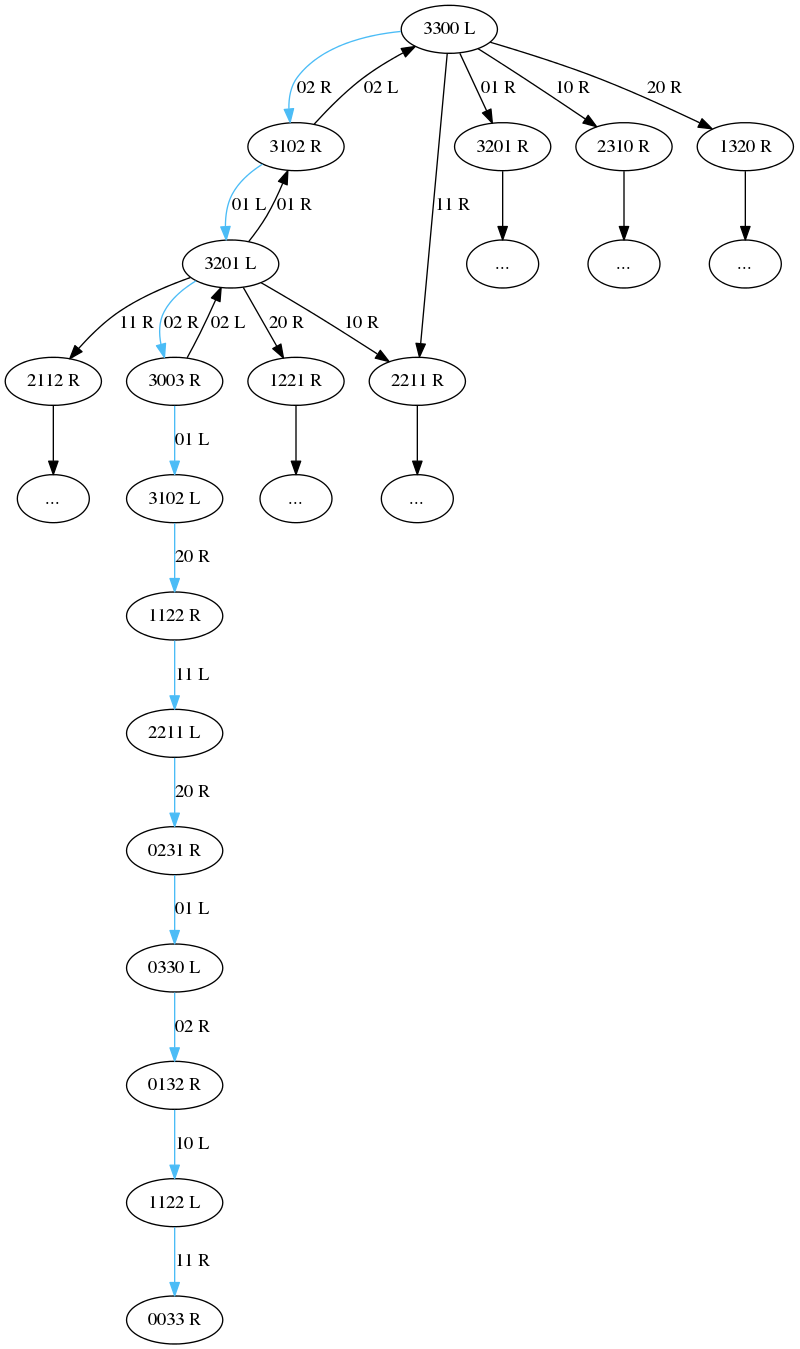
\includegraphics[width=0.65\textwidth]{./statespace.png}
  \caption{Partial State-Space Graph}
	\label{fig2}
\end{figure}

\end{document}
